\providecommand{\relativeRoot}{../..}
\documentclass[\relativeRoot/main.tex]{subfiles}
\graphicspath{
    {\subfix{./figures/}}
}

\begin{document}

\section{The lymphatic system}
\label{sec:intro:lymph_system}

\begin{figure}
    \centering
    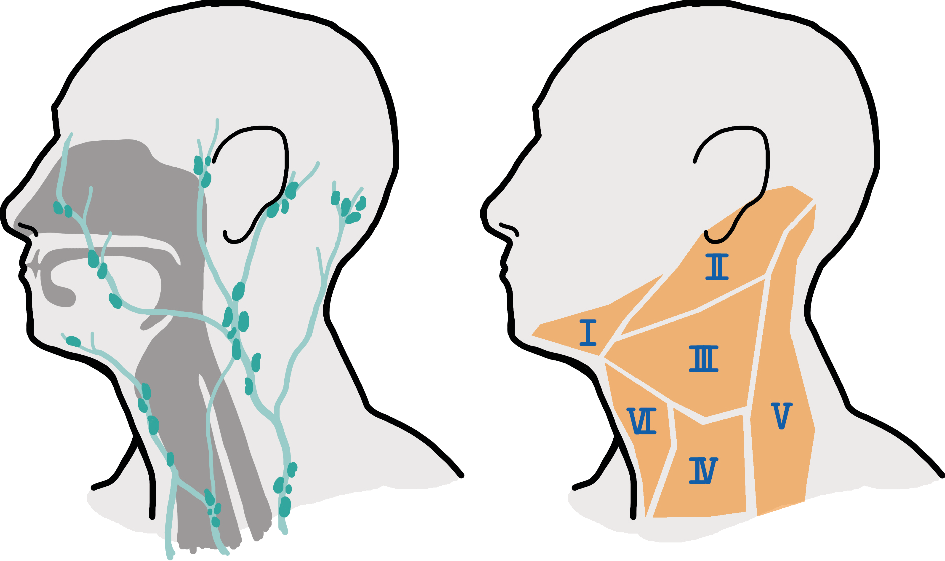
\includegraphics[width=\textwidth]{figures/schematics_head.pdf}
    \caption[
        Schematics of the head and neck regions with the anatomically defined LNLs
    ]{
        Schematic drawing of the head and neck region showing the respiratory system (gray), the lymphatic vessels (light green) and individual lymph nodes (green) in the left drawing. On the right, the rough outlines of the \acrshortpl{lnl} of the head and neck are overlaid. LNL VII is not visible on this schematic but is located right below LNL VI. These schematics are roughly traced from Lengelé et al. \cite{lengele_anatomical_2007}.
    }
    \label{fig:intro:schematics_head}
\end{figure}

\end{document}